\documentclass[tikz]{standalone}

\usepackage{xstring}

\usetikzlibrary{fit,positioning}


\begin{document}

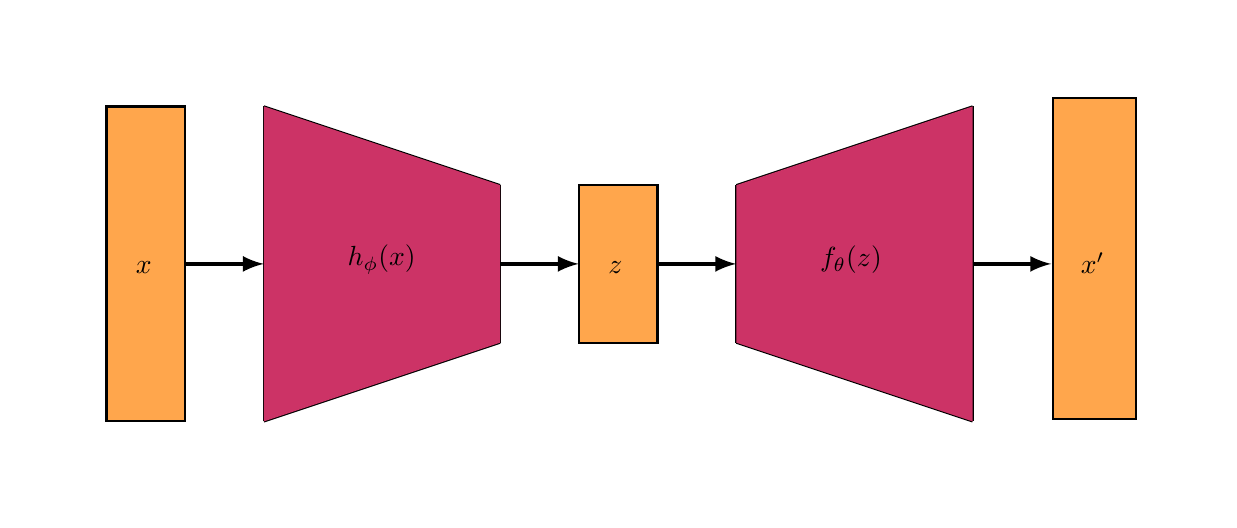
\begin{tikzpicture}
  \useasboundingbox (-9, -8) rectangle (6, -2);
	\draw[draw=black, fill=orange!70, thick, solid] (-8.00,-3.00) rectangle (-7.00,-7.00);
    
	\draw[draw=black, thick, solid] (-6.00,-3.00) -- (-6.00,-7.00);
	\draw[draw=black, thick, solid] (-6.00,-3.00) -- (-3.00,-4.00);
	\draw[draw=black, thick, solid] (-6.00,-7.00) -- (-3.00,-6.00);
	\draw[draw=black, thick, solid] (-3.00,-6.00) -- (-3.00,-4.00);

        \fill[fill=purple!80] 
    (-6.00,-3.00) -- (-6.00,-7.00) -- (-3.00,-6.00) -- (-3.00,-4.00) -- cycle;
    
	\draw[draw=black, fill=orange!70, thick, solid] (-2.00,-4.00) rectangle (-1.00,-6.00);
    
	\draw[draw=black, thick, solid] (0.00,-4.00) -- (0.00,-6.00);
	\draw[draw=black, thick, solid] (0.00,-6.00) -- (3.00,-7.00);
	\draw[draw=black, thick, solid] (3.00,-7.00) -- (3.00,-3.00);
	\draw[draw=black, thick, solid] (3.00,-3.00) -- (0.00,-4.00);

    \fill[fill=purple!80]
    (0.00,-4.00) -- (0.00,-6.00) -- (3.00,-7.00) -- (3.00,-3.00) -- cycle;
    
	\draw[draw=black, fill=orange!70, thick, solid] (4.02,-2.89) rectangle (5.08,-6.97);
    
	\draw[draw=black, -latex, ultra thick, solid] (-7.00,-5.00) -- (-6.00,-5.00);
	\draw[draw=black, -latex, ultra thick, solid] (-3.00,-5.00) -- (-2.00,-5.00);
	\draw[draw=black, -latex, ultra thick, solid] (-1.00,-5.00) -- (0.00,-5.00);
	\draw[draw=black, -latex, ultra thick, solid] (3.00,-5.00) -- (4.00,-5.00);
    
    
	\node[black, anchor=south west] at (-5.06,-5.25) {$h_\phi(x)
$};
	\node[black, anchor=south west] at (0.94,-5.25) {$f_\theta(z)
$};
	\node[black, anchor=south west] at (-1.75,-5.25) {$z
$};
	\node[black, anchor=south west] at (-7.75,-5.25) {$x
$};
	\node[black, anchor=south west] at (4.25,-5.25) {$x'
$};
\end{tikzpicture}
\end{document}